\section{Signed barriers and the quenched interface limit}
\label{sec:interface}

By Proposition~\ref{prop:physical-criticality}, the common tuning parameter is
$\beta_* =\beta_c^\rho(\varepsilon)$.  We now use the finite-vector
comparison of Proposition~\ref{prop:torus-tests} to place the target
interface between two pure comparison interfaces.  The comparisons
will preserve the pure marginal conditional on the original bond
environment.  This is the property that will yield convergence of
quenched laws, rather than only convergence after averaging over bonds.
Throughout this section, probabilities without an environmental
subscript include spins and coupling randomness as well as bonds.

\subsection{Boundary conventions and signed geometry}

Fix a bounded Jordan domain $D$, distinct marks $a,b\in\partial D$,
and the deterministic approximations in Theorem~\ref{thm:main}.
Write $D_n$ for their domains in physical coordinates, after
multiplication by $\delta_n$.  A lattice Jordan domain here is a full
square-lattice domain: bonds have not been deleted in its interior.
One standard convention surrounds the union of closed square cells
centered at the free spin sites, fixes the exterior nearest neighbors,
and retains every bond incident to a free spin.  The interface then
has a local half-edge at each boundary change.  Equivalently one can
use a lattice polygon made of plaquettes, with the boundary vertices
pinned and all interior vertices free.  The argument below applies to
both conventions.  In the first convention the exterior pin assignment
is an actual assignment to sites, so repeated incidences at one site
must have the same value.  The marked boundary changes and any
half-edge endpoints differ by at most $O(\delta_n)$.

We may take the boundary homeomorphisms to match the marks exactly.
Indeed, their inverse images of the discrete marks converge to $a,b$;
in a fixed circle parametrization, precompose by circle homeomorphisms
converging uniformly to the identity and taking $a,b$ to those inverse
images.  After passage to a subsequence the designation of the plus
arc is fixed.  Denote the open limiting arcs by $I_+$ and $I_-$.
Thus boundary order and signs, as well as positions, converge.
Winding number stability then implies that each compact subset of $D$
is eventually inside $D_n$, and each compact subset of
$\C\setminus\overline D$ is eventually outside $D_n$.

Let $\Gamma_n$ be the target contour, oriented from the mark near $a$
to the mark near $b$.  Its conditional law given the original
environment $\omega$ is $Q_{n,\omega}$.  We use the prescribed NE/SW
resolution, or a simple drawing of the same resolution inside small
vertex disks.  Matching the contour pieces in their traversal order
changes $d_{\rm curv}$ by $O(\delta_n)$.  The resolved graph has degree
two except at its two marked ends, so this drawing of its connecting
component is a simple arc.  Spin paths use the fixed triangulation by
NW/SE diagonals from the crossing section.  In the bulk its zero
contours have precisely these resolved connections.

We next describe the boundary placements used in
\cite[Section~9, ``Displaced domains and finite boundary barriers'']{R}
and \cite[Section~7, ``Fixed displaced domains and their boundary
incidences'']{S}.  To obtain the lower pure comparison, move the middle
plus boundary outward and the minus boundary inward.  Two cuts allow
comparison through a torus: a plus crossing screens the comparison
domain's plus boundary, and a minus crossing screens the target's minus
boundary.  After revealing these crossings, the remaining boundary
incidences have the orders needed for two comparisons with identical
couplings.  The strips on the central side of both cuts will transfer
signed barriers between the domains.

Fix a plane Schoenflies homeomorphism $\Psi$ taking
the unit disk to $D$, $1,-1$ to $a,b$, and the upper semicircle to
$I_+$.  These coordinates describe topology only; all tests below are
polygonal tests in the physical plane.

For small $h>0$, first take a radial boundary equal to $1+3h$ on
$[4h,\pi-4h]$, equal to $1-3h$ off $(3h,\pi-3h)$, and affine on
the two intervening angular intervals.  Its image under $\Psi$
encloses a preliminary domain favoring minus.  Put its marks at angles
$6h,\pi-6h$, and give the intervening upper arc the plus sign.  The
remaining arc is minus.  A minus cutting corridor $C_h^-$ follows
$\rho=1-h$ on $[\pi-h,2\pi+h]$, bending outward at its ends past
$\rho=1+h$; it is outside this comparison domain.  A plus corridor
$C_h^+$ follows $\rho=1+h$ from $5h$ to $\pi-5h$, bending outward
at its ends past $1+4h$.  It is outside $D$, and its caps cross the
minus shoulders of the comparison boundary.  Give the corridors small
positive widths and slightly larger, mutually disjoint reveal regions
on their exterior sides.  Their caps extend beyond the boundaries they
cut.  The minus reveal region stays outside the comparison domain;
the plus reveal region stays outside $\overline D$.
The \emph{central side} of a cut means its side toward $\Psi(0)$.

Replace this finite configuration by sufficiently close polygonal
arcs in the physical plane, preserving order, the cap crossings, and
all the stated positive clearances.  Such approximations can be made
inside the transported rectangular neighborhoods of the arcs; this is
the deterministic construction in the cited section of~\cite{S}.
Call the polygonal domain $A_h^-$ and its marks $a_h^-,b_h^-$.
Choose the approximation errors to vanish with $h$.  Its boundary
parametrizations therefore converge uniformly to those of $D$.
Rotating the coordinate construction by $\pi$ and interchanging signs
gives a domain $A_h^+$ favoring plus, still oriented from the mark
near $a$ to that near $b$.

An \emph{allowed plus strip} is a polygonal topological rectangle
whose closure lies inside $A_h^-$, on the central side of both cuts,
and is disjoint from the closed reveal regions.  Its two end gates lie outside $\overline D$
on the enlarged plus side.  Its closure stays in
$\Psi(\{\rho<1+h/2\})$ with a positive margin.  All its contacts
with $\partial D$ lie on $I_+$, away from the marks.  In a target
sample a plus crossing of the strip is tested by filling its portions
outside $D_n$ virtually with plus.  This specifies a geometric event;
it changes no actual spin or Gibbs weight.  Minus strips in $A_h^+$
are defined with the signs reversed.  Figure~\ref{fig:strip-squeeze}
distinguishes the cutting corridors from the strips they will protect.

\begin{figure}[tbp]
 \centering
 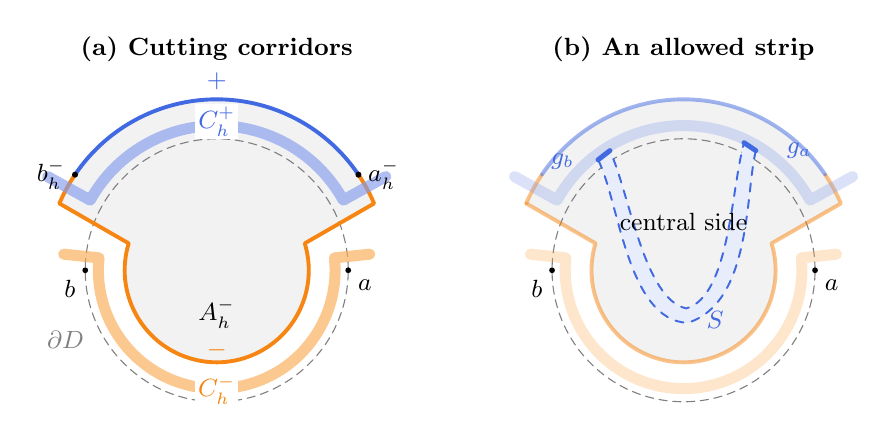
\begin{tikzpicture}[scale=1.67,line cap=round,line join=round,
  every node/.style={font=\small},
  plus/.style={draw=RoyalBlue,line width=1.4pt},
  minus/.style={draw=BurntOrange,line width=1.4pt},
  cutplus/.style={draw=RoyalBlue!65,line width=4pt,opacity=.65},
  cutminus/.style={draw=BurntOrange!65,line width=4pt,opacity=.65}]
\begin{scope}
  \node[font=\small\bfseries] at (0,1.68) {(a) Cutting corridors};
  \fill[gray!10] (23:1.30) arc[start angle=23,end angle=157,radius=1.30]
    -- (163:.70) arc[start angle=163,end angle=377,radius=.70] -- cycle;
  \draw[densely dashed,gray] (0,0) circle[radius=1];
  \draw[minus] (157:1.30)--(163:.70)
    arc[start angle=163,end angle=377,radius=.70]--(23:1.30)
    arc[start angle=23,end angle=34,radius=1.30];
  \draw[minus] (146:1.30) arc[start angle=146,end angle=157,radius=1.30];
  \draw[plus] (34:1.30) arc[start angle=34,end angle=146,radius=1.30];
  \draw[cutplus] (29:1.47)--(29:1.10)
    arc[start angle=29,end angle=151,radius=1.10]--(151:1.47);
  \draw[cutminus] (174:1.17)--(174:.90)
    arc[start angle=174,end angle=366,radius=.90]--(366:1.17);
  \node[RoyalBlue,fill=white,inner sep=1pt] at (0,1.13) {$C_h^+$};
  \node[BurntOrange,fill=white,inner sep=1pt] at (0,-.91) {$C_h^-$};
  \node at (0,-.33) {$A_h^-$};
  \node[gray] at (-1.15,-.53) {$\partial D$};
  \fill (1,0) circle[radius=.022] node[below right] {$a$};
  \fill (-1,0) circle[radius=.022] node[below left] {$b$};
  \fill (34:1.30) circle[radius=.023] node[right] {$a_h^-$};
  \fill (146:1.30) circle[radius=.023] node[left] {$b_h^-$};
  \node[RoyalBlue] at (0,1.44) {$+$};
  \node[BurntOrange] at (0,-.61) {$-$};
\end{scope}
\begin{scope}[xshift=3.55cm]
  \node[font=\small\bfseries] at (0,1.68) {(b) An allowed strip};
  \fill[gray!10] (23:1.30) arc[start angle=23,end angle=157,radius=1.30]
    -- (163:.70) arc[start angle=163,end angle=377,radius=.70] -- cycle;
  \draw[densely dashed,gray] (0,0) circle[radius=1];
  \draw[minus,opacity=.5] (157:1.30)--(163:.70)
    arc[start angle=163,end angle=377,radius=.70]--(23:1.30)
    arc[start angle=23,end angle=34,radius=1.30];
  \draw[minus,opacity=.5] (146:1.30) arc[start angle=146,end angle=157,radius=1.30];
  \draw[plus,opacity=.5] (34:1.30) arc[start angle=34,end angle=146,radius=1.30];
  \draw[cutplus,opacity=.3] (29:1.47)--(29:1.10)
    arc[start angle=29,end angle=151,radius=1.10]--(151:1.47);
  \draw[cutminus,opacity=.3] (174:1.17)--(174:.90)
    arc[start angle=174,end angle=366,radius=.90]--(366:1.17);
  \path[fill=RoyalBlue!12,draw=RoyalBlue,dashed,line width=.7pt]
    (.55,.91)..controls (.47,.60) and (.52,-.25)..(.03,-.40)
    ..controls (-.43,-.38) and (-.49,.53)..(-.65,.84)
    --(-.56,.91)
    ..controls (-.41,.58) and (-.30,-.22)..(.02,-.29)
    ..controls (.35,-.20) and (.36,.61)..(.46,.97)--cycle;
  \draw[plus,line width=1.8pt] (.55,.91)--(.46,.97);
  \draw[plus,line width=1.8pt] (-.65,.84)--(-.56,.91);
  \node[RoyalBlue] at (.88,.91) {$g_a$};
  \node[RoyalBlue] at (-.92,.83) {$g_b$};
  \node[RoyalBlue] at (.24,-.38) {$S$};
  \node at (0,.37) {central side};
  \fill (1,0) circle[radius=.022] node[below right] {$a$};
  \fill (-1,0) circle[radius=.022] node[below left] {$b$};
\end{scope}
\end{tikzpicture}

 \caption{Schematic geometry in Schoenflies coordinates for the
 minus-favoring comparison.  The dashed circle represents
 $\partial D$.  The boundary of $A_h^-$ is enlarged along its middle
 plus arc and moved inward elsewhere.  The blue cutting corridor is
 outside $D$; its caps cross the minus shoulders of $A_h^-$.  The
 orange corridor is outside $A_h^-$ and cuts off the target minus
 arc.  In the second panel an allowed plus strip lies on the central
 side of both cuts, with gates outside $D$.  Widths and displacements
 are exaggerated.  The strip is a deterministic test region, not a
 sampled interface, and the physical construction uses polygonal
 approximations.}
 \label{fig:strip-squeeze}
\end{figure}

At each fixed $h$ these placements are valid for every sufficiently
large $n$.  Boundary winding controls the compact clearances, and the
marked boundary order controls signs near each contact.  The caps
prevent paths from going around the ends of a cut.  This remains true
for a free path ending next to an exterior pin: append its final
incident bond before applying separation.  With pinned boundary
vertices that last bond already lies in the polygon.  The difference
between the two conventions is contained in one lattice layer and
cannot defeat a fixed-clearance cap.

\subsection{Conditioning at a fixed environment}

For laws of vectors in $\{0,1\}^m$, write $\preceq$ for stochastic
order with respect to coordinatewise order.  We record the elementary
coupling fact from \cite[Section~9, Lemma ``Conditioning and gluing at
fixed environment'']{R}, including its proof because its conditional
marginal is essential here.

\begin{lemma}[Conditional gluing]
\label{lem:conditional-gluing}
Let $\lambda$ be a deterministic law on a finite set and $\mu_\omega$
a measurable environmental family of laws on another finite set.
Let $U,W$ be vector-valued functions on these sets with values in
$\{0,1\}^m$.  Suppose $p,q_\omega$ are laws of
$(e,v)\in\{0,1\}\times\{0,1\}^m$, with $q_\omega$ measurable,
$p$ deterministic, and
$p(e=1)\ge c>0$, such that
\[
 \mathcal L_\lambda(U)\preceq p(v\in\cdot\mid e=1),\qquad
 q_\omega(v\in\cdot\mid e=1)\preceq\mathcal L_{\mu_\omega}(W)
\]
whenever the second conditional law is defined.  There is a measurable
coupling $\pi_\omega$ of $\lambda,\mu_\omega$ satisfying
\[
 \E_{\rm env}\pi_\omega\{U\npreceq W\}
 \le \frac{6}{c}\E_{\rm env}\|p-q_\omega\|_{\TV}.
\]
In particular its first marginal is $\lambda$ in every environment.
\end{lemma}

\begin{proof}
Put $e_\omega=\|p-q_\omega\|_{\TV}$.  On $e_\omega\le c/2$,
$q_\omega(e=1)\ge c/2$, and subtraction of the conditional fractions
gives
\[
 \|p(v\in\cdot\mid e=1)-q_\omega(v\in\cdot\mid e=1)\|_{\TV}
 \le 4e_\omega/c.
\]
Couple these middle vectors maximally and glue to the two order
couplings.  Extend the outer vectors to complete samples using their
conditional laws given $U,W$.  Order fails only when the middle
vectors disagree.  On $e_\omega>c/2$ use any coupling with the same
prescribed marginals; this exceptional set has probability at most
$2\E_{\rm env}e_\omega/c$.  This proves the bound.  All required
couplings are measurable finite-dimensional kernels: enumerate the
finitely many linear-programming bases of each coupling problem and
select the first feasible basic solution.  Subsequent conditional
probabilities are explicit finite ratios, with a fixed arbitrary
probability law on each zero-mass fiber.
\end{proof}

The environment has not been conditioned on $e=1$.  We condition spin
laws separately at each fixed environment, including when deciding
which environments require an arbitrary coupling.

\begin{proposition}[Transfer of a finite strip family]
\label{prop:strip-transfer}
Fix $h>0$ and a finite family of allowed plus strips in $A_h^-$.
The pure critical Dobrushin sample in an ordinary mesh approximation
of $A_h^-$ and the target sample in $D_n$ admit couplings conditional
on the original environment such that every strip crossed by plus in
the pure sample is crossed by plus in the virtually filled target,
with annealed probability $1-o(1)$.  The pure marginal conditional on
the original environment is its deterministic pure law.  The analogous
assertion holds for minus strips in $A_h^+$.
\end{proposition}

\begin{proof}
Embed the target and comparison domains, their incident bond layers,
the two corridors, their reveal regions, and the strips in a torus
chart with a fixed positive buffer.  Use the target bond
environment in that chart and independent bonds to complete the
torus, whose period is chosen as in Proposition~\ref{prop:torus-tests}.
Until the final averaging step include those extra bonds in the environment.
Let $E_h$ be the event of the two required cutting crossings, and
$V$ the vector of ordinary plus strip crossings in the torus.  For
the pure and quenched torus vector laws $p_n,q_{n,\omega}$,
\begin{equation}
 p_n(E_h)\ge c_h>0,\qquad
 \E_{\rm env}\|p_n-q_{n,\omega}\|_{\TV}\longrightarrow0.
 \label{eq:strip-middle-laws}
\end{equation}
The first assertion is the pure buffered RSW construction for two
disjoint prescribed-color corridors
\cite[Section~2, Proposition ``Pure buffered RSW consequences'']{S};
the second is Proposition~\ref{prop:torus-tests}, applied to the
fixed finite vector $(\1_{E_h},V)$.  No comparison of the entire
torus spin configurations is asserted.

We verify the two stochastic orders needed for
Lemma~\ref{lem:conditional-gluing}.  In either torus conditioned on
$E_h$, inspect each corridor from its exterior side, stopping at its
first crossing of the required color.  The construction is
\cite[Section~6, Lemma ``Reveals with a monochromatic facing
boundary'']{S}.  It can be described by querying the inspecting
boundary and expanding the queried cluster of the opposite color.
Every unqueried neighbor of that cluster is queried; queried vertices
of the required color are not expanded.  On success the facing
boundary is the required monochromatic crossing, and nothing beyond
it toward the center is queried.  Planarity of the triangulation
gives this facing crossing; the cap extensions ensure that every
nearest-neighbor incidence across the explored side meets one of
its pins.  The two reveal regions are disjoint.

For clarity, an adaptive stopped reveal has exactly the required
conditional law.  Its next queried site and its stopping decision are
functions of the preceding answers.  A completed transcript
$(v_1,s_1),\ldots,(v_k,s_k)$ therefore occurs precisely when those
queried spins have those values.  Conditioning on the transcript
pins those spins and imposes no further restriction.  Since the
transcripts determine $E_h$, conditioning on $E_h$ adds nothing once
the transcripts are specified.

In the first comparison, the lower law is pure Dobrushin in $A_h^-$
and the upper law is the pure torus conditioned on $E_h$.  In the
union of the whole common nearest-neighbor free components containing
the strip portions on the central side, the revealed plus path
is an upper plus pin against a lower free site.  It screens the
comparison domain's plus boundary.  All remaining accessible domain
boundary incidences are lower minus pins against upper free sites.
At a meeting they are upper plus against lower minus.  The minus
reveal is outside $A_h^-$.  Thus the pure-domain strip vector is
below $p_n(V\in\cdot\mid E_h)$.

In the second comparison, the lower law is the quenched torus
conditioned on $E_h$ and the upper law is the target.  Again use the
whole common nearest-neighbor free components containing the interior
strip portions on the central side.  Now the minus
path screens the target minus boundary, and the plus reveal is
outside the target.  With the upper entry first, the incidences are
\[
 (+,\mathrm{free}),\qquad (\mathrm{free},-),\qquad (+,-).
\]
All bonds incident to common free vertices have identical couplings
in the two laws being compared.  Condition on the other spins.
Each displayed pair orders the resulting boundary fields, regardless
of the value of a free site in that pair.  The nearest-neighbor
ferromagnetic boundary comparison therefore orders the conditional
spin laws; averaging over these other spins preserves the order.
This argument takes place at fixed environment and uses only
$K_e(\beta_*)>0$.  It does not compare pure bond strengths with
random bond strengths.

The geometric incidence verification is precisely that of
\cite[Section~9, proof of ``Quenched transfer of a finite strip
family'']{R} and \cite[Section~7, proof of ``Fixed-geometry boundary
squeeze'']{S}.  A nearest-neighbor edge cannot cross a triangulated
path in the interior of an edge; the caps prevent an incidence from
escaping around a cut.  The marked clearances established above
exclude a wrongly signed accessible boundary pin.  These statements
also cover the last edge to an exterior pin and the boundary-vertex
convention.  Virtual plus values give the upper value on every
portion of a strip outside $D_n$.  We obtain, jointly for the entire
finite list,
\[
 \mathcal L(V_{A_h^-})\preceq p_n(V\in\cdot\mid E_h),\qquad
 q_{n,\omega}(V\in\cdot\mid E_h)\preceq\mathcal L_\omega(V_{D_n}).
\]
Lemma~\ref{lem:conditional-gluing} and
\eqref{eq:strip-middle-laws} give the result for vector laws and,
by disintegration, for full spin samples.  Average over the added
torus bonds conditional on the original environment.  The target
marginal never used those bonds, and the pure marginal remains its
fixed pure law.  The sign-reversed construction is identical.
\end{proof}

\subsection{From strips to ordered traces}

To use a virtually filled crossing as a barrier, one needs exact
noncrossing, rather than just two drawings at distance $O(\delta_n)$.
We give the boundary check from
\cite[Section~7, Lemma ``Local drawing beside a signed strip'']{S}.
For a fixed finite strip list, its boundary contacts lie on compact
signed arcs separated from the marks.  Near a plus contact every
exterior nearest neighbor of a free site is already plus.  Fill the
other exterior vertices of incident faces with plus for drawing
purposes.  In the cell convention, a boundary dual vertex meets one,
two adjacent, or three interior cells; two opposite cells alone would
violate the Jordan condition.  With one interior cell, the two
nearest exterior neighbors already have the filling sign, so filling
the opposite exterior corner changes no bond incident to that cell.
With two adjacent or three interior cells, all exterior corners are
already nearest neighbors.  Triangular interpolation consequently
preserves every target disagreement edge and every resolved local
connection.  With pinned boundary vertices the same assertion follows
directly by interpolating the plaquettes with their given arc values.

Redraw the target in the faces meeting the strips and one adjacent
layer using these zero segments.  They glue at the same edge
midpoints, preserve traversal order, and avoid all corresponding
monochromatic paths.  Plus and minus contact sets are separated, so
the two fillings can be made simultaneously.  The half-edge ends
and neighborhoods of the marks are untouched.  Denote the resulting
drawing by $\widetilde\Gamma_n$; then
\begin{equation}
 d_{\rm curv}(\widetilde\Gamma_n,\Gamma_n)=O(\delta_n),
 \qquad \widetilde\Gamma_n\text{ is disjoint from every selected barrier}.
 \label{eq:barrier-redrawing}
\end{equation}
This changes the drawing only, including in a domain with narrow
fjords: no exterior spin or incident interaction is removed.

We use the following pure geometric input from
\cite[Section~9, Lemma ``Finite strips and limiting barriers'']{R},
proved in \cite[Section~7, ``From fixed strip tests to limiting
barriers'']{S}.  Given $\eta_j\downarrow0$, one can choose
$h_j\downarrow0$ and a deterministic finite list of allowed strips
of each sign at displacement $h_j$ such that, outside pure
probability $O(\eta_j)$, a comparison chord selects a strip whose
end gates it crosses with strict margins.  Its omitted terminal
pieces have diameter at most $\eta_j$.  The strip has cross-sections
of diameter at most $\eta_j$ following a simple prototype within
$\eta_j$ in curve distance of the remaining subarc.  For sufficiently
fine ordinary lattice approximations the same assertion holds, with
errors $O(\eta_j)$, and the signed side of the lattice interface
supplies a monochromatic crossing of that strip.

Here are the relevant hypotheses and parameter order behind this
input.  The pure Dobrushin convergence to $\SLE_3$ is used only in a
fixed polygonal domain, with the full curve convergence supplied by
\cite{CDHKS,KS}; see also the pure input statements in~\cite{R,S}.
Uniform convergence of Jordan boundary parametrizations gives
uniform convergence on the closed disk of the normalized conformal
maps, by Rad\'o's domain-continuity theorem as stated and explained
in~\cite[Section~7, beginning of ``From fixed strip tests to limiting
barriers'']{S}.  In particular the hypotheses give a common boundary
local-connectedness modulus.  Uniform convergence transfers nearby
points on the varying boundaries to nearby points of the limiting
boundary; uniform continuity of the limiting inverse and of the
parametrizations then controls a joining boundary subarc.  The boundary
crosscut proof of the conformal extension theorem upgrades kernel
convergence using this modulus.  Thus boundary fjords do not require
an extra regularity assumption.  Mapping a single disk
$\SLE_3$ by those maps shows that the continuum laws in $A_h^\pm$
converge in the oriented curve metric to $\SLE_3(D;a,b)$ as
$h\downarrow0$.  Simplicity and avoidance of the boundary away from
the two endpoints imply that compact middle subarcs stay inside $D$.
In the enlarged domain, take the last and first hits of
$\rho=1+h/3$ around an interior point and extend slightly at their
ends.  These hits are on the enlarged signed side, outside $D$;
the extensions stay below $1+h/2$.  Polygonal tolerances are chosen
smaller than the gaps between these radial levels.  This gives the allowed gates,
and the omitted terminal diameters tend to zero.  Thin rectangular
neighborhoods of these simple subarcs can be chosen polygonal with
strict traversal margins.  Rational choices form a countable open
cover of the favorable curves; a finite subcover in probability
loses at most another $\eta_j$.  To see the signed crossing in a fine
lattice approximation, follow the selected interface traversal through
its successive interpolation triangles.  Their plus-side vertices
are connected by plus edges of those triangles, with common vertices
or edges across each consecutive face.  They form a plus walk at
distance $O(\delta_n)$ from the traversal.  The positive long-side
clearance keeps this walk inside the strip; the transverse crossing
margins carry it beyond both end gates.  Crop it at those gates and
erase loops.  Backtracking of the interface does not affect this
existence argument.  The entire finite list is fixed
before Proposition~\ref{prop:strip-transfer} is applied.  The sampled
curve chooses its strip only afterwards.

Choose increasing deterministic integers $n_j\ge j$ so that for
every $n\ge n_j$ all fixed-$j$ placements, pure approximation bounds,
and both strip transfers have errors at most $O(\eta_j)$, and the
pure comparison laws are within $\eta_j$ of their continuum laws in
bounded-Lipschitz distance.  Include the fixed-clearance exterior
closures described below among these requirements.  This absorbs
the possibly small $c_{h_j}$ in the conditional coupling estimate.
Set
\begin{equation}
 j(n)=\max\{j\le n:n_j\le n\}.
 \label{eq:interface-diagonal}
\end{equation}
Before $n_1$ make any choice.  Then $j(n)\to\infty$.
Let $L_n$ be the pure comparison chord in $A_{h_{j(n)}}^-$ and
$U_n$ the pure comparison chord in $A_{h_{j(n)}}^+$, both oriented
from the mark near $a$ to that near $b$.
Glue their couplings over the common pair consisting of the original
environment and target spin sample, by sampling the two conditional
comparison kernels given that pair.  Each comparison marginal
conditional on the original environment remains its deterministic
pure law.  Both marginal laws converge to $\SLE_3(D;a,b)$, and
with probability tending to one the target has both selected barriers.

All target traces eventually lie in a fixed compact planar disk.
The space of its nonempty compact subsets is compact in Hausdorff
distance.  Together with tightness of $L_n,U_n$ in the curve metric,
this gives, along any further subsequence, a joint subsequential limit
\[
 (\operatorname{tr}\Gamma_n,L_n,U_n)\Longrightarrow(K,L,U).
\]
Here $K$ is connected, contains $a,b$, and lies in $\overline D$;
these facts follow respectively from Hausdorff convergence,
endpoint convergence, and the boundary winding argument.
Both $L,U$ are simple $\SLE_3$ chords with interiors in $D$.
For such a chord $C$, let $P(C),M(C)$ denote the open components of
$D\setminus C$ adjacent to $I_+,I_-$, respectively.

The barriers imply
\begin{equation}
 K\subset\overline{M(L)}\cap\overline{P(U)},
 \label{eq:trace-squeeze}
\end{equation}
where closures are in $\overline D$.  We spell out why this includes
the open boundary arcs, following
\cite[Section~7, ``Forbidden sides, order, and identification of the
trace'']{S}.  Represent the subsequential convergence almost surely
and, after a further subsequence, make barrier failures summable.
Erase loops in a successful plus crossing, join its ends to the gate
centers within the exterior gate neighborhoods, and close it by
radial paths in $\Psi$ coordinates to a fixed circle $\rho=\rho_*>1$,
followed by its plus-side circular arc.  The added paths have positive
clearance from $\overline D$ at each fixed $j$; the thresholds $n_j$
ensure that they are outside $D_n$.  Both target marks are on the
zero-winding side: their outward escape paths lie beyond the ends
of the extended plus arc.  Exact disjointness in
\eqref{eq:barrier-redrawing} keeps the entire target on that side.

The closed path need not be simple; its winding number is constant
along any curve disjoint from it.  Every crossing between the strip gates is homotopic within the
rectangular strip, relative to its gates, to its prototype.  Thus
backtracking of that crossing cannot alter its winding about points
outside the strip.  Vanishing strip widths, prototype errors, and
terminal diameters make this winding equal eventually to the nonzero
winding of $L$ closed on the plus side, on each compact subset of
$P(L)$.  The fixed outer circular arc remains a positive distance
beyond each compact subarc of $I_+$, and the connectors tend to the
two endpoint connectors.  The same nonzero winding therefore holds
in a neighborhood of every point of $I_+$ other than $a,b$.
The target avoids all these neighborhoods.  Its limit lies in
$\overline{M(L)}$, and the minus barrier gives the other inclusion
in~\eqref{eq:trace-squeeze}.

\begin{lemma}[Ordered chords with equal laws]
\label{lem:ordered-chords}
Let $L,U$ be random simple chords from $a$ to $b$ with interiors in
$D$, and let $K\subset\overline D$ be random, compact, connected,
and contain $a,b$.  If \eqref{eq:trace-squeeze} holds, then
$P(L)\subset P(U)$ almost surely.  If $L,U$ have the same trace law,
then $K=L=U$ as compact sets almost surely.
\end{lemma}

\begin{proof}
This elementary planar argument is
\cite[Section~7, Lemma ``Ordered chords with equal laws'']{S}.
If $P(L)\cap M(U)$ were nonempty, a point in the intersection could
be joined inside these side domains to the two opposite open boundary
arcs.  Removing loops gives a crosscut between those arcs disjoint
from $K$, by~\eqref{eq:trace-squeeze}.  Its endpoints alternate
with $a,b$, so it separates $a$ from $b$, contradicting connectedness.
Thus $P(L)\subset P(U)\cup U$.  An interior point of $U$ cannot
lie in the open set $P(L)$, because every neighborhood of that point
meets $M(U)$.  Hence $P(L)\subset P(U)$.

Map to the disk by the fixed Schoenflies map and take the ordinary
areas of the two plus sides.  These bounded random variables are
ordered and have the same distribution, so their difference is zero
almost surely.  A proper inclusion of the side domains would give
positive area difference: a point in $P(U)\setminus P(L)$ is either
in $M(L)$, or on $L$, in which case its neighborhood in $P(U)$ meets
$M(L)$.  The difference therefore contains a nonempty open set.
The plus sides, and hence their interior boundary chords, are equal.
Finally \eqref{eq:trace-squeeze} puts $K$ on that chord.  Its inverse
parametrization sends $K$ to a connected subset of $[0,1]$ containing
both endpoints, necessarily all of $[0,1]$.  No zero-area assertion
about the chords was needed.
\end{proof}

Consequently every joint trace limit satisfies $K=L=U$.  It remains
to rule out repeated forward and backward traversal near this trace.

\subsection{Passages control traversal order}

The passage criterion below is proved in
\cite[Section~7, Lemma ``Progress coordinates and the full curve
metric'']{S}; we include its proof to make the passage from compact
sets to oriented curves explicit.  It uses the interior estimate
of Corollary~\ref{cor:four-passages}.  This is a concrete version
of the role of multiple-crossing bounds in curve compactness
arguments~\cite{AB,KS}.

\begin{lemma}[Progress along a simple limiting chord]
\label{lem:progress}
Suppose $g_n$ are simple oriented curves, their endpoints tend to
$a,b$, and their traces converge in Hausdorff distance to that of
an injective continuous chord $G:[0,1]\to\overline D$ with endpoints
$a,b$ and $G((0,1))\subset D$.  There are continuous
$u_n:[0,1]\to[0,1]$, with endpoint values tending to $0,1$, such that
\[
 e_n:=\sup_t|g_n(t)-G(u_n(t))|\longrightarrow0.
\]
If $B_n:=\sup_{s<t}(u_n(s)-u_n(t))\to0$, then
$d_{\rm curv}(g_n,G)\to0$.  Conversely, for each $0<\eta<1$,
a drop $B_n\ge\eta$ forces six disjoint passages from radius $r$
to radius $R_\eta>0$ about a point of
$G([\eta/2,1-\eta/2])$, for every $e_n<r<R_\eta$ and all
sufficiently large $n$.  Here $R_\eta$ depends only on $G,\eta$.

The corresponding convergence in probability holds for random
coupled curves if trace and endpoint convergence hold in probability
and, for every deterministic $F\Subset D$ and all sufficiently small
fixed $R>0$,
\begin{equation}
 \lim_{r\downarrow0}\limsup_n
 \Prob\{g_n\text{ has four passages from }r\text{ to }R
                     \text{ about some point of }F\}=0.
 \label{eq:progress-passage}
\end{equation}
Passages are counted on disjoint open parameter intervals.
\end{lemma}

\begin{proof}
Extend the continuous inverse coordinate $G^{-1}$ from its compact
trace continuously to an ambient neighborhood, with values in
$[0,1]$, and compose it with $g_n$.  Uniform continuity gives the
assertions about $u_n,e_n$ and their endpoints.  If $B_n\to0$,
the running maximum $m_n(t)=\max_{s\le t}u_n(s)$ satisfies
$0\le m_n(t)-u_n(t)\le B_n$.  Normalize its endpoint values to
$0,1$, obtaining a nondecreasing continuous $v_n$ with
$\|v_n-u_n\|_\infty\to0$.  For any $\kappa_n\downarrow0$ with
$\kappa_n>0$, the function
$h_n(t)=(1-\kappa_n)v_n(t)+\kappa_n t$ is an increasing
homeomorphism of $[0,1]$.  If $\omega_G$ is the modulus of
continuity of $G$, then
\[
 d_{\rm curv}(g_n,G)
 \le e_n+\omega_G(\|h_n-u_n\|_\infty)\longrightarrow0.
\]

If instead $u_n(s)-u_n(t)\ge\eta$ for some $s<t$, put
$c_n=(u_n(s)+u_n(t))/2\in[\eta/2,1-\eta/2]$.  Once endpoint
coordinate errors are less than $\eta/4$, each of $[0,s],[s,t],[t,1]$
has endpoints on opposite sides of $c_n$, at coordinate distance
at least $\eta/4$.  Each interval contains a visit to $c_n$.
Injectivity and compactness give
\[
 q_\eta=\min_{|v-w|\ge\eta/4}|G(v)-G(w)|>0,\qquad
 d_\eta=\dist(G([\eta/2,1-\eta/2]),\partial D)>0.
\]
Choose $R_\eta<\min(q_\eta,d_\eta)/4$.  For $e_n<R_\eta$,
the four anchor points at parameters $0,s,t,1$ are outside the
radius-$R_\eta$ disk about $G(c_n)$, whereas the three level visits
are within $e_n$ of its center.  Cropping the incoming and outgoing
pieces at the inner and outer hits gives two annular passages in
each interval.  Their open parameter intervals are disjoint, and
simplicity makes their spatial interiors disjoint.  Thus there are
six passages, in particular four.  Fixed-factor crops give the same
conclusion for square annuli if those are used in
Corollary~\ref{cor:four-passages}.

For the random assertion, use a measurable continuous representative
of $G$.  Measurable progress coordinates are obtained without choosing
a random extension: write
$\Delta_n=d_H(\operatorname{tr}g_n,\operatorname{tr}G)$,
$z_n=2\Delta_n+1/n$, and set
\[
 u_n(t)=
 \frac{\displaystyle\int_0^1 v\,(z_n-|g_n(t)-G(v)|)_+\,\dd v}
 {\displaystyle\int_0^1 (z_n-|g_n(t)-G(v)|)_+\,\dd v}.
\]
The denominator is positive, and this is continuous in $t$ and
jointly measurable.  Put
$\iota_G(r)=\sup\{|v-w|:|G(v)-G(w)|\le r\}$, which tends to
zero with $r$.  Parameters receiving positive weight have diameter
at most $\iota_G(2z_n)$, so
\[
 e_n\le z_n+\omega_G(\iota_G(2z_n))\longrightarrow0
\]
in probability; endpoint coordinate errors also tend to zero.
These statements follow almost surely along any subsequence on
which the trace and endpoint errors converge almost surely, and
hence in probability for the full sequence.

Fix $\eta>0$ and an exceptional probability $\zeta>0$.  Choose
deterministic $q,d>0$ with
$\Prob(q_\eta<q\text{ or }d_\eta<d)<\zeta$.  The random
centers then lie in the deterministic compact set
$F_d=\{z\in\overline D:\dist(z,\partial D)\ge d\}$.
Fix a deterministic $R<\min(q,d)/8$ small enough for
\eqref{eq:progress-passage}.  For every fixed $0<r<R$, the
six-passage argument bounds
\[
 \limsup_n\Prob(B_n\ge\eta)
 \le \zeta+\limsup_n\Prob\{\text{four passages about some point of }
                                      F_d\text{ from }r\text{ to }R\}.
\]
Let $r\downarrow0$ and then $\zeta\downarrow0$.  Thus
$B_n\to0$ in probability.  Localizing the random continuity
modulus $\omega_G$ outside another event of probability $\zeta$
and using the running-maximum construction gives the asserted
curve convergence.  All compact sets and radii used in the passage
estimate are deterministic before taking the mesh limit.
\end{proof}

\subsection{Completion of the main theorem}

\begin{proof}[Proof of Theorem~\ref{thm:main}]
The tuning, matching, and criticality arguments give
$\beta_* =\beta_c^\rho(\varepsilon)$ for all sufficiently small
fixed $\varepsilon>0$.  The tuning estimate
$\beta_*=K_0+O_\rho(\varepsilon^2)$ also gives the critical-temperature
estimate in the theorem.  Choose $\varepsilon_0(\rho)$ once to meet
their smallness conditions and the fixed-shape crossing bootstrap.
These choices precede every final domain, strip family, and
approximation sequence.

Begin with any subsequence of the deterministic approximations, and
pass further to fix the signed arc designation.  The slow diagonal
\eqref{eq:interface-diagonal} constructs couplings of the target and
two comparison chords satisfying
\[
 \mathcal L(\Gamma_n\mid\omega)=Q_{n,\omega},\qquad
 \mathcal L(L_n\mid\omega)=R_n,
 \qquad R_n\Longrightarrow\SLE_3(D;a,b),
\]
where $R_n$ is deterministic.  Every further subsequence has a joint
trace and comparison-curve limit, and the barrier argument and
Lemma~\ref{lem:ordered-chords} identify it as $(L,L,L)$ in traces.

We explain the probabilistic passage to curves without assuming
target curve tightness.  The space of continuous oriented curves
modulo zero uniform reparametrization distance is Polish.  Rational
polygonal paths are dense.  For completeness, select a Cauchy
subsequence with successive distances less than $2^{-j}$, choose
parametrized representatives $g_j$, and put $f_1=g_1$.  Given a
fixed representative $f_j$, choose increasing homeomorphisms
$\alpha,\beta$ such that
$\|f_j\circ\alpha-g_{j+1}\circ\beta\|_\infty<2^{1-j}$, and put
$f_{j+1}=g_{j+1}\circ\beta\circ\alpha^{-1}$.  Then
$\|f_{j+1}-f_j\|_\infty<2^{1-j}$.  The representatives converge
uniformly to a continuous path $f$, and
$d_{\rm curv}(f_j,f)\le\|f_j-f\|_\infty\to0$; the original
Cauchy sequence has the same limit.  Pauses are permitted in this
ambient continuous-curve space and removed by the zero-distance
identification when appropriate.  Thus the joint trace and comparison
convergence admits an almost surely convergent representation.
Lift that representation to target paths by their original
conditional laws given the trace and the two comparison curves.
At each mesh the target has finite configuration space, so these
kernels exist directly.  The lift preserves every joint law at
that mesh, and in particular every annealed target passage bound.

Corollary~\ref{cor:four-passages} gives
\eqref{eq:progress-passage} for these target curves: interior
charts have fixed free buffers, arbitrary exterior spins are allowed,
and target passages are bounded by the local event that any resolved
contours supply the required passages.  Local redrawings are absorbed
by fixed-factor radius crops.  Lemma~\ref{lem:progress} now gives
$d_{\rm curv}(\Gamma_n,L)\to0$ in probability in the representation.
Since also $L_n\to L$ in curve distance,
$d_{\rm curv}(\Gamma_n,L_n)\to0$ there and hence in the original
couplings.  Every further subsequence permits this argument, so it
holds along the chosen sequence.  In particular
\begin{equation}
 \E\min\{1,d_{\rm curv}(\Gamma_n,L_n)\}\longrightarrow0.
 \label{eq:quenched-coupling-error}
\end{equation}

Write $\bar d=\min\{1,d_{\rm curv}\}$.  For any test function
in the bounded-Lipschitz class for $\bar d$, the conditional coupling
and its two correct marginals give
\[
 \left|\int F\,\dd Q_{n,\omega}-\int F\,\dd R_n\right|
 \le \E\bigl[\bar d(\Gamma_n,L_n)\mid\omega\bigr].
\]
Taking the supremum over that class and then environmental expectation,
\begin{equation}
 \E_{\rm env}d_{\rm BL}(Q_{n,\omega},R_n)
 \le \E\bar d(\Gamma_n,L_n)\longrightarrow0.
 \label{eq:quenched-bl}
\end{equation}
The conditional pure marginal is essential in this step.  Measurability
holds also for a nonatomic bond law: at each mesh $Q_{n,\omega}$ has
a fixed finite curve support and measurable probabilities, and its
distance to a fixed law is a continuous function of these probabilities.
Added torus bonds and auxiliary coupling variables have already been
integrated out conditional on the original environment.

The deterministic laws $R_n$ converge in bounded-Lipschitz distance
to the stated SLE law.  Equation~\eqref{eq:quenched-bl}, the triangle
inequality, and Markov's inequality prove convergence in environmental
probability on the chosen subsequence.  If it failed for the original
sequence, a subsequence on which the failure probability stayed
positive would contradict this construction.  Finally restore the
prescribed lattice drawing and half-edges; their matched displacement
is $O(\delta_n)$, with the same orientation.  This proves the theorem
in the required uniform oriented-curve metric.
\end{proof}
